\scanpage{65}
\mspage{8}
et on a
\[
g(z)=\varphi g'(\psi(z))
\]
où $\varphi,\psi$ sont les transformations homographiques satisfaisant
\[
\psi:\left\{\begin{array}{c}1\\-1\\0,\infty\end{array}\right.
\longrightarrow
\left\{\begin{array}{c}0\\\infty\\1,-1\end{array}\right.
\qquad
\varphi:\left\{\begin{array}{cc}0&0\\\infty&1\\1&\infty\end{array}\right.
\]
donc \deleted{$\unsure{\varphi}$}
\[
\psi(z)=\frac{z-1}{z+1}\qquad
\varphi(z)=\sigma_0(z)=\frac{z}{z-1}
\]
d'où
\[
g(z)=\frac{\left(\frac{z-1}{z+1}\right)^2}{\left(\frac{z-1}{z+1}\right)^2+1}
=\frac{(z-1)^2}{(z-1)^2-(z+1)^2}
=\frac{(z-1)^2}{-4z}
\]
\[
\text{(23)}\qquad g(z)=-\frac1{4z}(z-1)^2
\]
réalise l'isomorphisme conforme du disque unité $\mathbb D$ sur la découpe $f$ de $\mathbb P^1(\mathbb C)$ suivant $[0,1]$, avec les valeurs annoncées plus haut...
\[
\text{---}
\]

Le groupe $\Pi_{0,3}^{\tau}$ apparaît comme groupe fondamental mixte
\[
\text{(24)}\qquad
\Pi_{0,3}^{\tau}\simeq\Pi_1(U_{0,3},\{1,\tau\};P_+)
\]
\margin{\uline{NB} \unsure{Ici}\quad
$\rho_i=\lambda_{i+1}^{\deleted{\unsure{-1}}}\lambda_{i-1}^{-1}$}

Introduisant les chemins \inserted{$\lambda_i\ (i\in\{0,1,\infty\})$} de $P_-$ à $P_+$, formés des demi-arcs de grand cercle passant par les $Q_i$ (\inserted{$Q_i$,} milieux des arcs de grand cercle joignant $j$ à $k$, où $\{i,j,k\}=\{0,1,\infty\}$), on aura, en tant que flèches de $\Pi_1(U_{0,3},\{1,\tau\})$ :
\[
\tau_i=\left(\underbrace{\lambda_i}_{\tau P_+=P_-\to P_+},
\underset{\substack{\unsure{\uparrow}\\\{1,\tau\}}}{\tau}\right)
\]
\figure{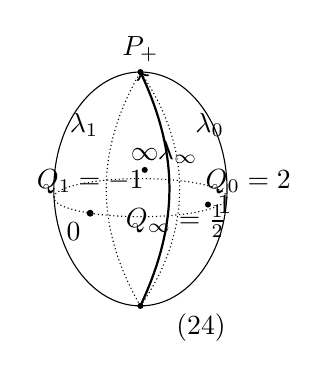
\begin{tikzpicture}[scale=1.1]
\draw (0,0) ellipse (1 and 1.35);
\draw[densely dotted] (0,-.1) ellipse (1 and .22);
\draw[densely dotted] (0,-1.35) to[out=120,in=-120] (0,1.35);
\draw[densely dotted] (0,-1.35) to[out=55,in=-55] (0,1.35);
\draw[thick,->] (0,-1.35) to[out=65,in=-65] (0,1.35);
\fill (0,1.35) circle (.035); \node[above] at (0,1.35) {$P_+$};
\fill (0,-1.35) circle (.035);
\fill (-.58,-.28) circle (.04); \node[below left] at (-.58,-.28) {$0$};
\fill (.78,-.18) circle (.035); \node[right] at (.78,-.18) {$1$};
\fill (.05,.22) circle (.035); \node[above] at (.05,.22) {$\infty$};
\node at (-.65,.74) {$\lambda_1$}; \node at (.8,.74) {$\lambda_0$};
\node at (.43,.43) {$\lambda_\infty$};
\node at (-.58,.08) {$Q_1=-1$}; \node[right] at (.64,.08) {$Q_0=2$};
\node at (.41,-.37) {$Q_\infty=\frac12$};
\node at (.7,-1.6) {(24)};
\end{tikzpicture}}
\margin{64}
